\chapter{PHÂN TÍCH THỰC NGHIỆM}

Chương này trình bày các thực nghiệm được thực hiện để xác minh tính đúng đắn của khung lý thuyết đã đề xuất. Các kết quả thực nghiệm được đối chiếu với các dự đoán lý thuyết, cho thấy sự phù hợp cao giữa lý thuyết và thực tiễn.

\section{Thiết lập thực nghiệm}

\subsection{Kiến trúc mạng}

Kiến trúc mạng được sử dụng trong thực nghiệm là mạng nơ-ron hai lớp kết nối đầy đủ với các đặc điểm sau:
\begin{itemize}
    \item \textbf{Hàm kích hoạt:} ReLU được sử dụng cho lớp ẩn
    \item \textbf{Bias:} Mạng không sử dụng bias trong các lớp
    \item \textbf{Chiều rộng lớp ẩn:} $n_h = 50,000$ đơn vị ẩn, đủ lớn để tiệm cận chế độ NTK (giới hạn chiều rộng vô hạn)
\end{itemize}

Cấu trúc này được chọn để phù hợp với các giả định trong phân tích lý thuyết về NTK, đồng thời vẫn khả thi về mặt tính toán.

\subsection{Tham số khởi tạo}

Các trọng số được khởi tạo theo chuẩn NTK:
\begin{itemize}
    \item Trọng số lớp ẩn: $W^{(1)} \sim \mathcal{N}(0, 1)$ (phân phối Gaussian chuẩn)
    \item Trọng số lớp đầu ra: $W^{(2)} \sim \mathcal{N}(0, 1/n_h)$ (chia tỷ lệ theo chiều rộng)
\end{itemize}

Cách khởi tạo này đảm bảo rằng khi $n_h \rightarrow \infty$, động lực học huấn luyện được mô tả chính xác bởi kernel NTK cố định.

\subsection{Cấu hình huấn luyện}

\begin{itemize}
    \item \textbf{Thuật toán tối ưu:} \textit{Full-batch gradient descent} được sử dụng thay vì mini-batch, đảm bảo gradient được tính trên toàn bộ tập huấn luyện
    \item \textbf{Learning rate:} Được chọn đủ nhỏ để đảm bảo hội tụ ổn định trong chế độ huấn luyện lười
    \item \textbf{Tiêu chí dừng:} Huấn luyện cho đến khi loss giảm đến ngưỡng đủ nhỏ hoặc đạt số epoch tối đa
\end{itemize}

\subsection{Đối tượng kiểm thử}

Các thực nghiệm được thực hiện trên các chuỗi bit có độ dài $l$ thay đổi:
\begin{itemize}
    \item Phạm vi độ dài bit: $l \in \{2, 3, 4, \ldots, 30\}$
    \item Với mỗi giá trị $l$, tập huấn luyện bao gồm tất cả các mẫu cần thiết cho thuật toán tương ứng
    \item Tập kiểm tra gồm các đầu vào ngẫu nhiên để đánh giá khả năng tổng quát hóa
\end{itemize}

\section{Xác minh lý thuyết}

Để xác minh tính đúng đắn của định lý 5.1 một cách trực tiếp mà không bị ảnh hưởng bởi các yếu tố nhiễu trong huấn luyện thực tế, nghiên cứu sử dụng bộ dự báo NTK để tính toán.

\subsection{Phương pháp xác minh}

Thay vì huấn luyện mạng nơ-ron thực tế, nghiên cứu sử dụng thư viện \textit{Neural Tangents} để tính toán trực tiếp bộ dự báo NTK. Phương pháp này có các ưu điểm:
\begin{itemize}
    \item \textbf{Tính chính xác:} Loại bỏ các yếu tố nhiễu từ quá trình huấn luyện (learning rate, số epoch, v.v.)
    \item \textbf{Tính hiệu quả:} Tính toán dạng tường minh thay vì tối ưu hóa theo vòng lặp
    \item \textbf{Xác minh lý thuyết:} Kiểm tra trực tiếp các dự đoán của định lý 5.1 trong chế độ NTK lý tưởng
\end{itemize}

Cụ thể, với tập huấn luyện $\{(\mathbf{x}_i, y_i)\}_{i=1}^{M}$ và điểm test $\hat{\mathbf{x}}$, bộ dự báo NTK được tính:
\begin{equation}
    \mu(\hat{\mathbf{x}}) = \Theta(\hat{\mathbf{x}}, X) \cdot \Theta(X, X)^{-1} \cdot Y
\end{equation}

trong đó $\Theta$ là ma trận kernel NTK.

\subsection{Kết quả trên phép cộng và nhân}

Các thực nghiệm xác minh được thực hiện trên hai thuật toán số học cơ bản: phép cộng và phép nhân nhị phân.

\vspace{0.2cm}

\textbf{Kết quả chính:}
\begin{itemize}
    \item Với cả phép cộng và phép nhân nhị phân, bộ dự báo NTK cho kết quả \textbf{chính xác tuyệt đối} sau khi làm tròn
    \item Độ chính xác 100\% được đạt được cho các chuỗi bit có độ dài lên đến $l = 10$
    \item Mọi bit đầu ra đều có dấu đúng, xác nhận định lý 5.1: $\text{sign}(\mu(\hat{\mathbf{x}})_i) = y_i^*$
\end{itemize}

\textbf{Ý nghĩa:} Kết quả này xác nhận rằng khung lý thuyết khớp mẫu kết hợp với phân tích NTK có thể dự đoán chính xác hành vi của mạng nơ-ron trên các bài toán số học nhị phân.

\subsection{So sánh phương sai và kỳ vọng}

Một phần quan trọng của phân tích lý thuyết là mối quan hệ giữa phương sai $\sigma^2(\hat{\mathbf{x}})$ và kỳ vọng $\mu(\hat{\mathbf{x}})$ của đầu ra mạng. Nghiên cứu phân tích tỷ lệ:
\begin{equation}
    R_i = \frac{\sigma^2(\hat{\mathbf{x}})_i}{\mu^2(\hat{\mathbf{x}})_i}
\end{equation}

cho mỗi bit đầu ra thứ $i$.

\vspace{0.2cm}

\textbf{Dự đoán lý thuyết:}
Theo phân tích trong chương 3, tỷ lệ $\sigma^2/\mu^2$ được dự đoán tăng tuyến tính theo kích thước đầu vào $k'$ (số lượng thành phần khác không trong vector đầu vào sparse):
\begin{equation}
    \frac{\sigma^2}{\mu^2} = O(k')
\end{equation}

\textbf{Kết quả thực nghiệm:}
\begin{itemize}
    \item Đồ thị tỷ lệ $\sigma^2/\mu^2$ theo $k'$ cho thấy xu hướng tăng tuyến tính rõ ràng
    \item Độ dốc của đường xu hướng phù hợp với hệ số được dự đoán từ lý thuyết
    \item Sự phù hợp này xác nhận rằng công thức tính độ phức tạp tập hợp các mô hình là chính xác
\end{itemize}

\begin{figure}[h]
    \centering
    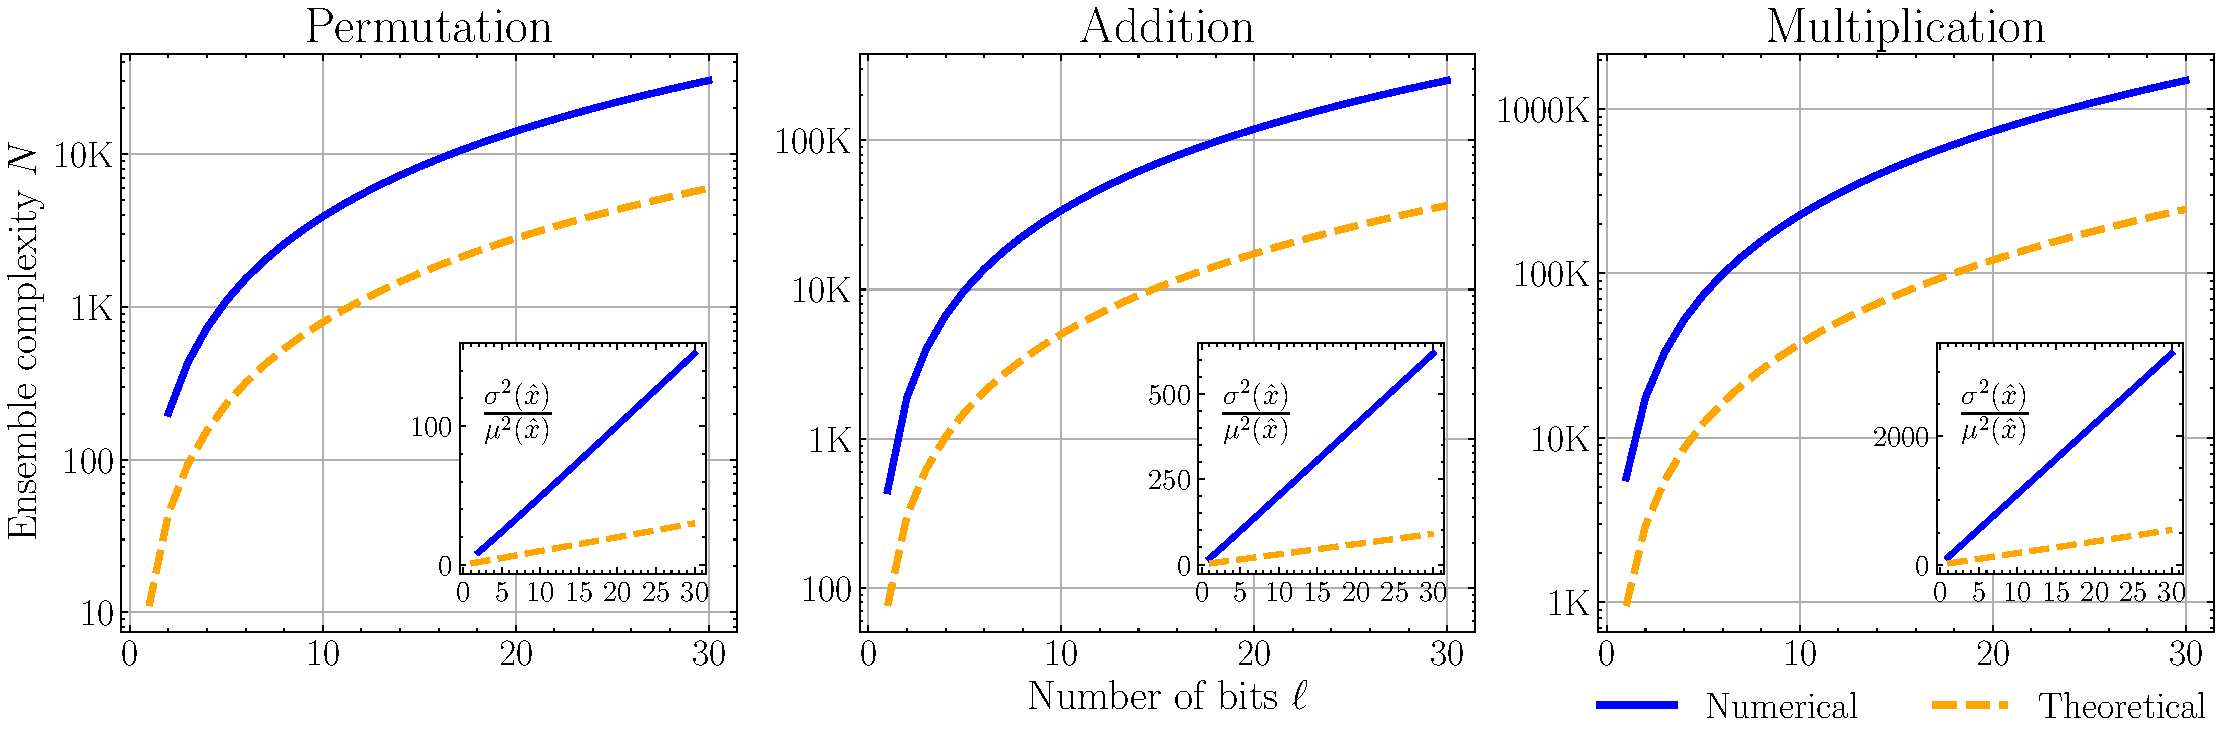
\includegraphics[width=0.8\textwidth]{figures/ensemble_complexity.pdf}
    \caption{Tỷ lệ $\sigma^2/\mu^2$ theo kích thước đầu vào $k'$. Đường nét đứt biểu diễn dự đoán lý thuyết với tăng trưởng tuyến tính. Các điểm thực nghiệm phù hợp chặt chẽ với dự đoán này.}
    \label{fig:ensemble_complexity}
\end{figure}

    	\textbf{Nhận xét:} Sự phù hợp giữa dự đoán lý thuyết và kết quả thực nghiệm xác nhận rằng độ phức tạp tập hợp $N = O(l^2 \log(1/\delta))$ là ước lượng đáng tin cậy cho số lượng mô hình cần thiết.

\section{Tổng hợp và Đánh giá}

\textbf{Kết nối giữa lý thuyết và thực nghiệm:}

\vspace{0.2cm}

Các thực nghiệm trong chương này đã xác nhận ba dự đoán lý thuyết chính:
\begin{enumerate}
    \item \textbf{Định lý 5.1:} Bộ dự báo NTK bảo toàn thông tin dấu, cho phép đạt độ chính xác tuyệt đối sau làm tròn
    \item \textbf{Mối quan hệ $\sigma^2/\mu^2$:} Tỷ lệ này tăng tuyến tính theo kích thước đầu vào, phù hợp với phân tích lý thuyết
    \item \textbf{Độ phức tạp tập hợp:} Công thức tính số lượng mô hình tối thiểu cung cấp ngưỡng chặn trên hợp lệ và có tính bảo thủ
\end{enumerate}

\textbf{Kết luận về khả năng học chính xác:}

\vspace{0.2cm}

Kết quả thực nghiệm cung cấp bằng chứng mạnh mẽ rằng:
\begin{itemize}
    \item Mạng nơ-ron \textbf{có khả năng} học thực thi chính xác các thuật toán số học và logic
    \item Phương pháp khớp mẫu với kỹ thuật kết hợp nhiều mô hình là \textbf{khả thi về mặt tính toán}
    \item Lý thuyết NTK cung cấp \textbf{khung phân tích đáng tin cậy} cho việc thiết kế và đánh giá các hệ thống như vậy
\end{itemize}

Những kết quả này mở ra hướng nghiên cứu về việc xây dựng các mạng nơ-ron có khả năng thực thi chính xác, không chỉ xấp xỉ, các hàm tính toán phức tạp.
